\documentclass[journal,onecolumn]{IEEEtran}

 \usepackage{cite}
\usepackage{amsmath,amsthm,amssymb}
\usepackage{graphicx}
\usepackage{siunitx}
\usepackage{multirow}
\usepackage{stfloats}
\usepackage{cases}
\usepackage{physics}
\usepackage{mathtools}
\sisetup{per-mode = symbol}
\newtheorem{theorem}{Theorem}
\newtheorem{lemma}{Lemma}
\newtheorem{proposition}{Proposition}
\newtheorem{definition}{Definition}
\usepackage{xcolor}
\newcommand{\rev}[1]{#1}% supplement: highlighting disabled (entire document is new R1 material)
\newcommand{\bI}{\mathbf{I}}
\newcommand{\bJ}{\mathbf{J}}
\newcommand{\tbJ}{\tilde{\bJ}}
\newcommand{\bH}{\mathbf{H}}
\newcommand{\bL}{\mathbf{L}}
\newcommand{\bM}{\mathbf{M}}
\newcommand{\bU}{\mathbf{U}}
\newcommand{\bE}{\mathbf{E}}
\newcommand{\bF}{\mathbf{F}}
\newcommand{\bP}{\mathbf{P}}
\newcommand{\bT}{\mathbf{T}}
\newcommand{\bp}{\mathbf{p}}
\newcommand{\bpi}{\mathbf{\pi}}
\newcommand{\bPi}{\mathbf{\Pi}}
\newcommand{\bq}{\mathbf{q}}
\newcommand{\bx}{\mathbf{x}}
\newcommand{\by}{\mathbf{y}}
\newcommand{\bY}{\mathbf{Y}}
\newcommand{\bz}{\mathbf{z}}
\newcommand{\bff}{\mathbf{f}}
\newcommand{\bg}{\mathbf{g}}
\newcommand{\bk}{\mathbf{k}}
\newcommand{\bl}{\mathbf{l}}
\newcommand{\bu}{\mathbf{u}}
\newcommand{\bv}{\mathbf{v}}
\newcommand{\bw}{\mathbf{w}}
\newcommand{\bphi}{\mathbf{\Phi}}
\newcommand{\Tbphi}{\Tilde{\bphi}}
\newcommand{\bxi}{\boldsymbol{\xi}}
\newcommand{\blam}{\boldsymbol{\Lambda}}
\newcommand{\tou}{\text{out}}
\newcommand{\ti}{\text{in}}
\newcommand{\tn}{\text{node}}
\newcommand{\tecp}{\text{cp}}
\newcommand{\ttb}{\text{tb}}
\newcommand{\tecc}{\text{cc}}
\newcommand{\D}{\text{D}}
\newcommand{\V}{\mathcal{V}}
\newcommand{\cB}{\mathcal{B}}
\newcommand{\cA}{\mathcal{A}}
\newcommand{\cC}{\mathcal{C}}
\newcommand{\cX}{\mathcal{X}}
\newcommand{\cY}{\mathcal{Y}}
\newcommand{\cZ}{\mathcal{Z}}
\newcommand{\cW}{\mathcal{W}}
\newcommand{\dm}{\dot{m}}
\newcommand{\dmin}{\dot{m}^\text{in}}
\newcommand{\Ts}{T^\text{s}}
\newcommand{\Tre}{T^\text{r}}
\newcommand{\Touts}{T^\text{out,s}}
\newcommand{\Toutr}{T^\text{out,r}}
\newcommand{\Vt}{\tilde{V}}
\newcommand{\cH}{\mathcal{H}}
\newcommand{\ipv}{i_\text{pv}}
\newcommand{\vpv}{v_\text{pv}}
\newcommand{\cpv}{C_\text{pv}}
\newcommand{\voc}{V_\text{oc}}
\newcommand{\isc}{I_\text{sc}}
\newcommand{\im}{I_\text{m}}
\newcommand{\vm}{V_\text{m}}
\newcommand{\rsun}{R_\text{sun}}
\newcommand{\il}{i_\text{L}}
\newcommand{\ldc}{L_\text{dc}}
\newcommand{\vdc}{v_\text{dc}}
\newcommand{\idc}{i_\text{dc}}
\newcommand{\kp}{k_\text{p}}
\newcommand{\ki}{k_\text{i}}
\newcommand{\vid}{v_\text{id}}
\newcommand{\viq}{v_\text{iq}}
\newcommand{\vix}{v_\text{ix}}
\newcommand{\viy}{v_\text{iy}}
\newcommand{\vrd}{v_\text{rd}}
\newcommand{\vrq}{v_\text{rq}}
\newcommand{\ix}{i_x}
\newcommand{\iy}{i_y}
\newcommand{\vx}{v_x}
\newcommand{\vy}{v_y}
\newcommand{\lf}{L_\text{f}}
\newcommand{\idref}{i_\text{dref}}
\newcommand{\iqref}{i_\text{qref}}
\newcommand{\kop}{k_\text{op}}
\newcommand{\koi}{k_\text{oi}}
\newcommand{\kip}{k_\text{ip}}
\newcommand{\kii}{k_\text{ii}}
\newcommand{\vdcref}{v_\text{dcref}}
\newcommand{\qref}{Q_\text{ref}}
\newcommand{\id}{i_d}
\newcommand{\iq}{i_q}
\newcommand{\vd}{v_d}
\newcommand{\vq}{v_q}
\newcommand{\ra}{r_\text{a}}
\newcommand{\xqp}{x_q'}
\newcommand{\xdp}{x_d'}
\newcommand{\edp}{e_d'}
\newcommand{\eqp}{e_q'}
\newcommand{\qr}{q_\text{R}}
\newcommand{\qt}{q_\text{T}}
\newcommand{\wref}{\omega_\text{ref}}
\newcommand{\qfuel}{q_\text{fuel}}
\newcommand{\qf}{q_\text{f}}
\newcommand{\sat}{\operatorname{Sat}}
\newcommand{\cop}{C_\text{op}}
\newcommand{\Pm}{P_\text{m}}
\newcommand{\pe}{P_\text{e}}
\newcommand{\DQ}{\Delta Q}
\newcommand{\dms}{\dot{m}^\text{s}}
\newcommand{\dmr}{\dot{m}^\text{r}}
\newcommand{\Vs}{\mathbb{V}^\text{s}}
\newcommand{\Vr}{\mathbb{V}^\text{r}}
\newcommand{\dH}{\Delta H}
\newcommand{\dHs}{\Delta H^\text{s}}
\newcommand{\dHr}{\Delta H^\text{r}}
\newcommand{\Hs}{H^\text{s}}
\newcommand{\Hr}{H^\text{r}}

% 天然气变量
\newcommand{\np}{p}
\newcommand{\nq}{q}
\newcommand{\bnq}{\boldsymbol{q}}

% 热力变量
\newcommand{\dht}{T}

\newcommand{\tih}{\tilde{h}}

% others
\newcommand{\jac}{Jacobian }
\newcommand{\te}{t_\text{end}}
\newcommand{\mcR}{\mathcal{R}}
\newcommand{\mcC}{\mathcal{C}}
\newcommand{\Tnab}{\Tilde{\nabla}}

\usepackage[hidelinks]{hyperref}
\hypersetup{
colorlinks=True,
citecolor=blue,
linkcolor=black
}

% Number sections, equations, figures, and tables with an "S" prefix so the
% main manuscript can refer to "Section S1", "Eq. (S5)", etc.
\renewcommand{\thesection}{S\arabic{section}}
\renewcommand{\theequation}{S\arabic{equation}}
\renewcommand{\thefigure}{S\arabic{figure}}
\renewcommand{\thetable}{S\arabic{table}}

\begin{document}
\title{Supplementary Material for\\ ``Acceleration of Gas-to-Power Cascading Fault Simulation Using Variable-Order-Variable-Step Numerical Differentiation Formulae''}
\author{Ruizhi~Yu,~Wei~Gu%
    \thanks{The authors are with the School of Electrical Engineering, Southeast University, Nanjing, Jiangsu, 210096 China. \emph{Corresponding author: Wei Gu}, e-mail: wgu@seu.edu.cn.}%
}
\maketitle

\noindent This document is the supplementary material accompanying the manuscript ``Acceleration of Gas-to-Power Cascading Fault Simulation Using Variable-Order-Variable-Step Numerical Differentiation Formulae''. Section, equation, figure, and table numbers carry the prefix ``S''. Cross-references of the form ``Section~S$n$ of the supplementary material'' in the main manuscript point to the correspondingly numbered section below.

\section{Selection of the NDF damping coefficient}
\label{app:kappa_selection}

\rev{The coefficient $\kappa$ is fixed for each order.
It is selected by combining the leading local-error constant with the root-locus stability boundary.
From the truncation-error expansion of the NDF-$k$ formula in the main manuscript, the leading error constant is}
\begin{equation}\label{eq:app_kappa_error_constant}
\rev{C_k(\kappa)=\qty|\frac{1}{k+1}+\kappa\gamma_k|,\quad
\gamma_k=\sum_{j=1}^{k}\frac{1}{j}.}
\end{equation}
\rev{For a prescribed error tolerance, the leading term satisfies $C_k(\kappa)h^{k+1}\approx \mathrm{constant}$.
Hence the asymptotic step-ratio relative to BDF-k is}
\begin{equation}\label{eq:app_kappa_step_ratio}
\rev{\chi_k(\kappa)=\qty(\frac{C_k(0)}{C_k(\kappa)})^{\frac{1}{k+1}}.}
\end{equation}

\rev{The accuracy target is determined from the second-order formula, because this is the highest order in the selected family for which A-stability can be retained.
For the selected coefficient, the formula is in fact L-stable, as shown below.
The stability calculation below shows that NDF-2 is A-stable exactly when}
\begin{equation}\label{eq:app_kappa_second_order_interval}
\rev{-\frac{1}{9}\leq\kappa\leq\frac{1}{3}.}
\end{equation}
\rev{On the negative branch, $C_2(\kappa)=1/3+3\kappa/2$ decreases as $\kappa$ decreases.
The unconstrained zero of this leading constant is $\kappa=-2/9$, which violates \eqref{eq:app_kappa_second_order_interval}.
Therefore the best second-order choice under the A-stability constraint is}
\begin{equation}\label{eq:app_kappa_second_order}
\rev{\kappa_2=-\frac{1}{9},\quad C_2(\kappa_2)=\frac{1}{6}.}
\end{equation}
\rev{Since $C_2(0)=1/3$, the corresponding step-ratio target is}
\begin{equation}\label{eq:app_kappa_chi_star}
\rev{\chi_\star=\qty(\frac{C_2(0)}{C_2(\kappa_2)})^{\frac{1}{3}}=2^{\frac{1}{3}}=1.2599.}
\end{equation}
\rev{We use this same leading-error step-ratio target for orders one and three.
Solving $\chi_k(\kappa_k)=\chi_\star$ on the negative branch gives}
\begin{equation}\label{eq:app_kappa_formula}
\rev{\kappa_k=\frac{2^{-\frac{k+1}{3}}-1}{(k+1)\gamma_k}.}
\end{equation}
\rev{For $k=1,2,3$, \eqref{eq:app_kappa_formula} gives}
\begin{equation}\label{eq:app_kappa_selected_values}
\rev{\kappa_1=-0.1850,\quad
\kappa_2=-\frac{1}{9},\quad
\kappa_3=-0.08225.}
\end{equation}

\rev{It remains to verify stability.
Apply the NDF-k formula to the scalar test equation $y'=\lambda y$ and set $z=h\lambda$.
If $r$ is an amplification root, then}
\begin{equation}\label{eq:app_kappa_stability_polynomial}
\rev{\sum_{m=1}^{k}\frac{1}{m}\qty(1-r^{-1})^m
-\kappa\gamma_k\qty(1-r^{-1})^{k+1}=z.}
\end{equation}
\rev{The boundary of the absolute-stability region is obtained by setting $r=\exp(\mathrm{i}\psi)$, $c=\cos\psi$, and $u=\sin\psi$.
Let $\delta=1-\exp(-\mathrm{i}\psi)$.
Then}
\begin{equation}\label{eq:app_kappa_root_locus}
\rev{z_k(\psi;\kappa)=\sum_{m=1}^{k}\frac{\delta^m}{m}
-\kappa\gamma_k\delta^{k+1}.}
\end{equation}
\rev{For the selected coefficients, the formulas are zero-stable at $z=0$: the principal root is $r=1$, and the largest moduli of the parasitic roots for orders one, two, and three are $0.1562$, $0.3163$, and $0.4871$, respectively.
Near $r=1$, $z=\delta+\order{\delta^2}$ and $\delta=1-r^{-1}=r-1+\order{(r-1)^2}$, so the principal root satisfies $r(z)=1+z+\order{z^2}$.
For sufficiently small negative real $z$, the principal root moves inside the unit disk, while the parasitic roots remain inside by continuity.
Thus the stable side of the root-locus boundary is the side containing the negative real axis near the origin.
If the boundary remains in the closed right half-plane, the full left half-plane is contained in the stability region.}

\rev{For $k=1$, the real part of \eqref{eq:app_kappa_root_locus} is}
\begin{equation}\label{eq:app_kappa_first_order_boundary}
\rev{\Re z_1=(1-c)(1+2\kappa c).}
\end{equation}
\rev{Thus $\Re z_1\geq0$ for every $c\in[-1,1]$ when $-1/2\leq\kappa\leq1/2$.
The selected value $\kappa_1=-0.1850$ lies in this interval, so the first-order formula is A-stable.}

\rev{For $k=2$, the real part is}
\begin{equation}\label{eq:app_kappa_second_order_boundary}
\rev{\Re z_2=(1-c)^2\qty[1+3\kappa(2c+1)].}
\end{equation}
\rev{Therefore $\Re z_2\geq0$ for every $c\in[-1,1]$ exactly when \eqref{eq:app_kappa_second_order_interval} holds.
The selected value $\kappa_2=-1/9$ lies at the accuracy-optimal A-stable endpoint.}

\rev{The selected first- and second-order formulas are further L-stable.
Indeed, write $\delta=1-r^{-1}$ in \eqref{eq:app_kappa_stability_polynomial}.
For $k=1$ and $k=2$, the selected $\kappa_k$ values are nonzero, so the highest-degree term $-\kappa_k\gamma_k\delta^{k+1}$ has a nonzero coefficient.
Hence $|\delta|\to\infty$ as $|z|\to\infty$ for every amplification root.
Since $r=(1-\delta)^{-1}$, all amplification roots satisfy $r\to0$ at infinity.
Together with the A-stability shown above, this proves L-stability of the selected first- and second-order formulas.}

\rev{For $k=3$, the boundary is not confined to the closed right half-plane, so the formula is not A-stable.
The real and imaginary parts of \eqref{eq:app_kappa_root_locus} are}
\begin{align}
\rev{x_3(c;\kappa)}
&\rev{=\frac{(1-c)^2}{3}\qty(1-4c+22\kappa-44\kappa c^2),}\label{eq:app_kappa_third_order_real}\\
\rev{y_3(c,u;\kappa)}
&\rev{=\frac{u}{3}\qty[8-9c+4c^2+44\kappa c(1-c)^2].}\label{eq:app_kappa_third_order_imag}
\end{align}
\rev{A-stability would require $1-4c+22\kappa-44\kappa c^2\geq0$ for all $c\in[-1,1]$.
Taking $c=0$ gives $\kappa\geq-1/22$, while taking $c=1$ gives $\kappa\leq-3/22$.
These two requirements are incompatible, so no third-order member of this one-parameter NDF family is A-stable.}
\rev{The half-angle of the stability wedge around the negative real axis is therefore}
\begin{equation}\label{eq:app_kappa_stability_angle}
\rev{\alpha_3(\kappa)=
\min_{c:\,x_3(c;\kappa)<0}
\tan^{-1}\qty(\frac{|y_3(c,\sqrt{1-c^2};\kappa)|}{-x_3(c;\kappa)}).}
\end{equation}
\rev{Substituting $\kappa_3=-0.08225$ into \eqref{eq:app_kappa_stability_angle} gives the minimizing point $c=0.28906$ and}
\begin{equation}\label{eq:app_kappa_third_order_angle}
\rev{\alpha_3(\kappa_3)=80.42^\circ.}
\end{equation}
\rev{Thus the selected third-order formula sacrifices full A-stability, which no third-order formula in this root-locus calculation attains, but it retains a broad $A(\alpha)$ stability wedge while matching the leading-error step-ratio target in \eqref{eq:app_kappa_chi_star}.}

\section{Numerical Dispersion in the Spatial Discretization of the Gas-Network PDEs}
\label{app:numerical_dispersion}

\rev{Traditional finite difference methods are stated in the problem formulation to introduce spurious numerical oscillations into the gas-network discretization.
These oscillations arise from the spatial discretization of the gas-network partial differential equations and are a manifestation of numerical dispersion.
They are distinct from the electromechanical oscillations of the synchronous machines.
A single-pipe leakage test is used to provide direct evidence for this statement and to justify the high-order non-oscillatory WENO3 discretization adopted in this work.}

\rev{The test pipe has length \SI{51}{\kilo\metre}, diameter \SI{0.5901}{\metre}, and friction factor $0.03$.
A source maintains a fixed pressure of \SI{6.62}{\mega\pascal} at the inlet, and the outlet draws a fixed load of \SI{14}{\kilogram\per\second}.
A leakage hole with diameter ratio $d/D=0.9$ opens at the pipe midpoint over \SI{5}{\second}, starting at $t=\SI{100}{\second}$.
Four spatial discretizations are compared: the central difference method (CDM) of second order, the first-order Euler upwind scheme, the first-order Kurganov-Tadmor (KT) scheme with the total variation diminishing property, and the third-order WENO3 scheme.
The benchmark is the method of characteristics with $\Delta x=\SI{100}{\metre}$ and $\Delta t=\SI{0.2942}{\second}$.
All four schemes under test use $\Delta x=\SI{500}{\metre}$, and the CDM and Euler schemes are integrated at $\Delta t=\SI{5}{\second}$.}

\begin{figure}[!t]
    \centering
    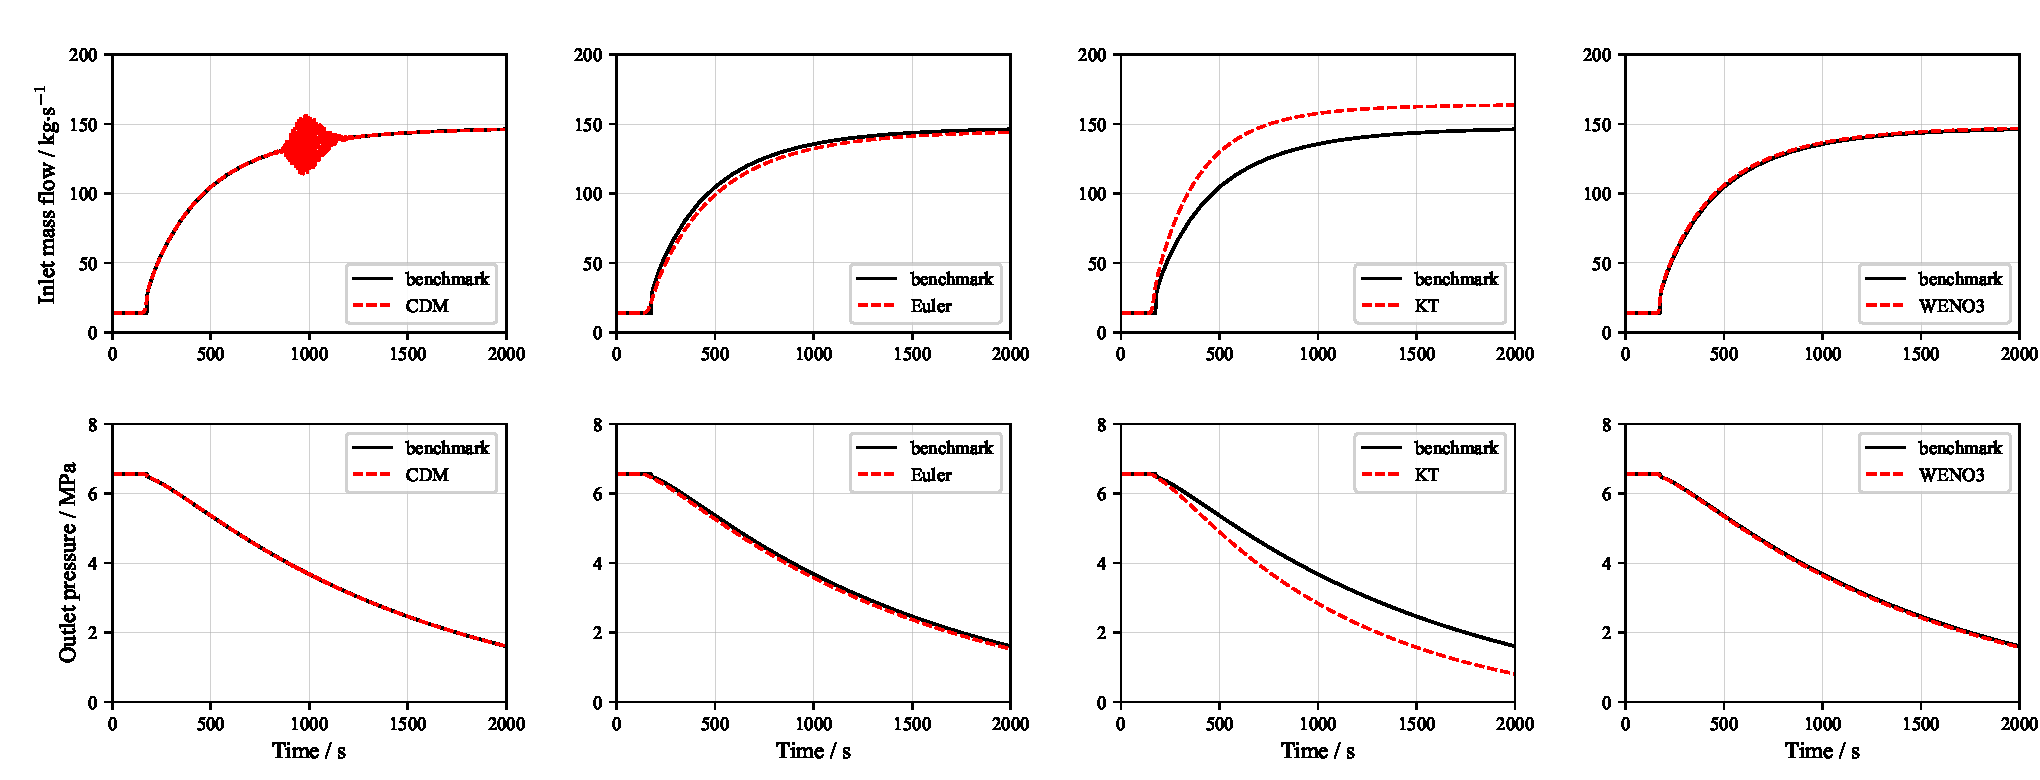
\includegraphics[width=\textwidth]{fig/leak_oscillation.pdf}
    \caption{\rev{Inlet mass flow and outlet pressure during the single-pipe leakage fault, computed by four spatial discretization schemes and compared with the method-of-characteristics benchmark. The second-order central difference method produces nonphysical oscillations in the inlet mass flow, while the third-order WENO3 scheme remains non-oscillatory and tracks the benchmark.}}
    \label{fig: leak_oscillation}
\end{figure}

\rev{Fig.~\ref{fig: leak_oscillation} shows the inlet mass flow $q_\ti$ and the outlet pressure $p_\tou$.
As gas feeds the leak, the inlet mass flow increases from its pre-fault value of \SI{14}{\kilogram\per\second} to approximately \SI{146}{\kilogram\per\second}, and the inlet begins to respond near $t=\SI{175}{\second}$, consistent with the \SI{75}{\second} acoustic travel time from the midpoint leak.
The CDM result exhibits a burst of nonphysical oscillations in the inlet mass flow between approximately $t=\SI{850}{\second}$ and $t=\SI{1150}{\second}$, with an amplitude up to about \SI{20}{\kilogram\per\second}.
These oscillations are purely numerical, since the second-order central scheme is dispersive at the steep gradient produced by the leak, and they could mislead an operator about the severity and timing of the fault.
The Euler and KT schemes suppress the oscillations through numerical dissipation but, being first order, are inaccurate.
The Euler result lags the benchmark throughout the transient, and the KT result overshoots the steady inlet mass flow to \SI{163.7}{\kilogram\per\second} and over-predicts the outlet pressure drop, falling to \SI{0.81}{\mega\pascal} against the benchmark value of \SI{1.60}{\mega\pascal}.
WENO3 is simultaneously non-oscillatory and accurate, tracking the benchmark in both quantities.}

\begin{table}[!h]
\centering
\setlength{\tabcolsep}{6pt}
\caption{\rev{Relative RMSE for the Single-Pipe Leakage Case}}\label{tb: leak_rmse}
\rev{\begin{tabular}{lccc}
\hline
Scheme & Spatial order & RMSE($q_\ti$) & RMSE($p_\tou$) \\ \hline
CDM    & 2 & $4.73\times10^{-2}$ & $1.96\times10^{-3}$ \\
Euler  & 1 & $5.50\times10^{-2}$ & $3.07\times10^{-2}$ \\
KT     & 1 & $1.95\times10^{-1}$ & $2.76\times10^{-1}$ \\
WENO3  & 3 & $2.92\times10^{-2}$ & $1.15\times10^{-2}$ \\ \hline
\end{tabular}}
\end{table}

\rev{Table~\ref{tb: leak_rmse} reports the relative root mean square error (RMSE) against the benchmark.
WENO3 attains the smallest inlet-flow error among the four schemes, whereas the first-order KT scheme yields the largest errors in both quantities, consistent with its pronounced overshoot in Fig.~\ref{fig: leak_oscillation}.
These results confirm that a high-order non-oscillatory discretization is required to avoid the numerical dispersion of the central difference method while retaining the accuracy that the dissipative low-order schemes sacrifice, which supports the WENO3 discretization adopted in this work.}

\section{Electric Power System Component Models}
\label{app:eps_models}

\rev{This appendix specifies the electric power system component models used in the case study: a sixth-order round-rotor machine with an AVR Type 1 dc exciter, a Type 2 power system stabilizer (PSS), and a Rowen gas-turbine governor, a current-injection network, and constant-power loads.
All quantities are in per unit and time constants in seconds; $\omega$ is the rotor speed, $V_t$ the terminal-voltage magnitude, $E_{fd}$ the field voltage, $v_s$ the PSS output, $u_x,u_y$ the rectangular bus voltage, and $\operatorname{sat}(x,a,b)=\min(\max(x,a),b)$.}

\rev{\textit{1) Synchronous machine:}
The sixth-order GENROU model, in the Sauer-Pai formulation\cite{sauerPowerSystemDynamics2018} and the implementation of\cite{cuiHybridSymbolicNumericFramework2021}, is}
\begin{equation}\label{eq:app_gen_swing}
\rev{\dot{\delta}=\omega_s(\omega-1), \qquad
\dot{\omega}=\frac{T_{\mathrm{m}}-T_e-D(\omega-1)}{2H},}
\end{equation}
\begin{equation}\label{eq:app_gen_emf}
\rev{\begin{aligned}
\dot{E}'_q&=\frac{1}{T'_{d0}}\big[-E'_q-(X_d-X'_d)(I_d-\gamma_d\eta_d)+E_{fd}-S_e E''_q\big],\\
\dot{E}'_d&=\frac{1}{T'_{q0}}\big[-E'_d+(X_q-X'_q)(I_q-\gamma_q\eta_q)-S_e g_{qd} E''_d\big],\\
\dot{\psi}_{1d}&=\frac{1}{T''_{d0}}\big[-\psi_{1d}+E'_q-(X'_d-X_l)I_d\big],\\
\dot{\psi}_{2q}&=\frac{1}{T''_{q0}}\big[-\psi_{2q}-E'_d-(X'_q-X_l)I_q\big],
\end{aligned}}
\end{equation}
\rev{with the subtransient EMFs, the $dq$/$xy$ Park transform, the stator equations, the electromagnetic torque, and the terminal voltage}
\begin{equation}\label{eq:app_gen_emfpp}
\rev{E''_q=a_d E'_q+b_d\psi_{1d}, \qquad E''_d=a_q E'_d-b_q\psi_{2q},}
\end{equation}
\begin{equation}\label{eq:app_gen_park}
\rev{\begin{aligned}
v_d&=u_x\sin\delta-u_y\cos\delta, & v_q&=u_x\cos\delta+u_y\sin\delta,\\
i_x&=I_d\sin\delta+I_q\cos\delta, & i_y&=I_q\sin\delta-I_d\cos\delta,\\
\end{aligned}}
\end{equation}
\begin{equation}\label{eq:app_gen_stator}
\rev{\begin{aligned}
v_d&=-R_a I_d+X''_q I_q+E''_d,\\
v_q&=-R_a I_q-X''_d I_d+E''_q,\\
\end{aligned}}
\end{equation}
\begin{equation}\label{eq:app_gen_te}
\rev{T_e=E''_d I_d+E''_q I_q+(X''_q-X''_d)I_d I_q, \quad V_t^2=v_d^2+v_q^2,}
\end{equation}
\rev{and the field saturation}
\begin{equation}\label{eq:app_gen_sat}
\rev{\begin{aligned}
S_e(\psi_{ag})&=B_s\frac{[\max(\psi_{ag}-A_s,0)]^2}{\psi_{ag}},\\
\psi_{ag}&=\sqrt{(E''_d)^2+(E''_q)^2},
\end{aligned}}
\end{equation}
\rev{where $\delta,\omega,E'_q,E'_d,\psi_{1d},\psi_{2q}$ are the rotor angle, per-unit speed, transient EMFs and damper-winding fluxes, $I_d,I_q$ and $v_d,v_q$ the $dq$-axis stator currents and voltages, $\eta_d=\psi_{1d}+(X'_d-X_l)I_d-E'_q$, $\eta_q=\psi_{2q}+(X'_q-X_l)I_q+E'_d$, $\gamma_d=(X'_d-X''_d)/(X'_d-X_l)^2$, $\gamma_q=(X'_q-X''_q)/(X'_q-X_l)^2$, $g_{qd}=(X_q-X_l)/(X_d-X_l)$, $a_d=(X''_d-X_l)/(X'_d-X_l)$, $b_d=(X'_d-X''_d)/(X'_d-X_l)$, $a_q=(X''_q-X_l)/(X'_q-X_l)$, $b_q=(X'_q-X''_q)/(X'_q-X_l)$, and $S_e$ the quadratic field-saturation function with coefficients $A_s,B_s$.}

\rev{\textit{2) Governor and prime mover:}
The Rowen gas-turbine model\cite{rowenSimplifiedMathematical1983} has seven states}
\begin{equation}\label{eq:app_gt_ode}
\rev{\begin{aligned}
\dot{T}_{ri}&=\frac{K_2 T_e-T_{ri}}{T_1}, &
\dot{T}_x&=\frac{T_r-T_x}{T_2}, \\
\dot{C}_{op}&=\frac{q_f-C_{op}}{T_{CD}}, &
\dot{q}_R&=\frac{W(\omega_{\mathrm{ref}}-\omega)-q_R}{T_G}, \\
\dot{x}_v&=\frac{q_{\mathrm{fuel}}-x_v}{b}, &
\dot{q}_f&=\frac{x_v-q_f}{T_{FS}}, \\
\end{aligned}}
\end{equation}
\begin{equation}\label{eq:app_gt_awu}
\rev{\dot{q}_{T,i}=
\begin{cases}
0, & q_T\geq q_{\max}\ \text{and}\ T_{\mathrm{ref}}-T_x\geq0,\\
0, & q_T\leq q_{\min}\ \text{and}\ T_{\mathrm{ref}}-T_x\leq0,\\
T_{\mathrm{ref}}-T_x, & \text{otherwise},
\end{cases}}
\end{equation}
\rev{the last a conditional-integration anti-windup; the algebraic outputs are}
\begin{equation}\label{eq:app_gt_alg}
\rev{\begin{aligned}
T_e&=T_{R0}+D(1-q_f)+E(1-\omega),\\
T_r&=K_1 T_e+T_{ri},\\
q_T&=k_i q_{T,i}+k_p(T_{\mathrm{ref}}-T_x),\\
T_{\mathrm{m}}&=A+B\,C_{op}+C(1-\omega),
\end{aligned}}
\end{equation}
\begin{equation}\label{eq:app_gt_fuel}
\rev{q_{\mathrm{fuel}}=k_{NL}+(1-k_{NL})\,\omega\,\min\!\big(q_T,\ \operatorname{sat}(q_R,q_{\min},q_{\max})\big),}
\end{equation}
\rev{where $T_{ri},T_x$ are the radiation-shield and thermocouple states, $C_{op}$ the compressor discharge, $q_R$ the governor signal, $x_v,q_f$ the valve and fuel-system states, $q_{T,i}$ the temperature-controller integrator, $T_e,T_r$ the exhaust and radiation-shield temperatures, $q_T$ the temperature-controller output, and the $\min$ in \eqref{eq:app_gt_fuel} the low-value fuel gate; $q_{\mathrm{fuel}}$ drives the gas-network draw.}

\rev{\textit{3) Automatic voltage regulator:}
The four-state AVR Type 1 dc exciter\cite{milanoPowerSystemModelling2010} is}
\begin{equation}\label{eq:app_avr}
\rev{\begin{aligned}
\dot{V}_{\mathrm{m}}&=\frac{V_t-V_{\mathrm{m}}}{T_r}, \\
e&=K_a\Big(V_{\mathrm{ref}}-V_{\mathrm{m}}-V_{r2}-\tfrac{K_f}{T_f}E_{fd}\Big)-V_{r}, \\
\dot{V}_{r}&=\frac{1}{T_a}\operatorname{awu}(V_{r},V_{r\min},V_{r\max},e), \\
\dot{V}_{r2}&=-\frac{1}{T_f}\Big(\tfrac{K_f}{T_f}E_{fd}+V_{r2}\Big), \\
\dot{E}_{fd}&=-\frac{1}{T_e}\Big(E_{fd}\big(K_e+S_e(E_{fd})\big)-V_{r}\Big),
\end{aligned}}
\end{equation}
\rev{with transducer state $V_{\mathrm{m}}$, amplifier state $V_{r}$, rate-feedback state $V_{r2}$, exciter field-voltage output $E_{fd}$, reference $V_{\mathrm{ref}}=V_{\mathrm{ref0}}+v_s$, and exciter saturation $S_e(E_{fd})=A_e\exp(B_e|E_{fd}|)$. The amplifier state carries an anti-windup limiter $\operatorname{awu}(\cdot)$ of the conditional-integration form in \eqref{eq:app_gt_awu} that holds $V_{r}$ within $[V_{r\min},V_{r\max}]$.}

\rev{\textit{4) Power system stabilizer:}
The three-state Type 2 PSS\cite{milanoPowerSystemModelling2010} feeds the rotor speed through the gain $K_w$, a washout, and two lead-lag stages:}
\begin{equation}\label{eq:app_pss}
\rev{\begin{aligned}
\dot{x}_{0}&=-\frac{K_w\omega+x_{0}}{T_w}, & y_{0}&=K_w\omega+x_{0}, \\
\dot{x}_{1}&=\frac{y_{0}-x_{1}}{T_2}, & y_{1}&=x_{1}+\tfrac{T_1}{T_2}(y_{0}-x_{1}), \\
\dot{x}_{2}&=\frac{y_{1}-x_{2}}{T_4}, & y_{2}&=x_{2}+\tfrac{T_3}{T_4}(y_{1}-x_{2}), \\
\end{aligned}}
\end{equation}
\begin{equation}\label{eq:app_pss_out}
\rev{v_s=\operatorname{sat}(y_{2},\ v_{s\min},\ v_{s\max}),}
\end{equation}
\rev{with washout state $x_{0}$ and output $y_{0}$, lead-lag states $x_{1},x_{2}$ and outputs $y_{1},y_{2}$. The washout removes the steady component of $K_w\omega$, and the output is clamped to $[v_{s\min},v_{s\max}]$.}

\rev{\textit{5) Network:}
With the bus admittance matrix $\mathbf{Y}=\mathbf{G}+\mathrm{j}\mathbf{B}$ from the power flow\cite{milanoPowerSystemModelling2010}, the current injection $I_i=i_{x,i}+\mathrm{j}\,i_{y,i}$ at bus $i$ is}
\begin{equation}\label{eq:app_network}
\rev{\begin{aligned}
i_{x,i}&=\sum_{j}\big(G_{ij}u_{x,j}-B_{ij}u_{y,j}\big), \\
i_{y,i}&=\sum_{j}\big(G_{ij}u_{y,j}+B_{ij}u_{x,j}\big),
\end{aligned}}
\end{equation}
\rev{summed over all buses $j$ and closed by the balance $I_i=I_i^{\mathrm{gen}}-I_i^{\mathrm{load}}$ of the machine stator and load currents at bus $i$.}

\rev{\textit{6) Load:}
Each static load is constant power\cite{milanoPowerSystemModelling2010}, with the floored squared voltage magnitude and rectangular current}
\begin{equation}\label{eq:app_load_veff}
\rev{|V_{\mathrm{eff}}|^2=\operatorname{sat}\!\big(u_x^2+u_y^2,\ v_{\min}^2,\ v_{\max}^2\big),}
\end{equation}
\begin{equation}\label{eq:app_load}
\rev{i_x=\frac{P_d u_x+Q_d u_y}{|V_{\mathrm{eff}}|^2}, \qquad
i_y=\frac{P_d u_y-Q_d u_x}{|V_{\mathrm{eff}}|^2}.}
\end{equation}
\rev{where $P_d,Q_d$ are the demand and the clamp $|V_{\mathrm{eff}}|^2$ holds the load at constant power within $[v_{\min},v_{\max}]$ and at constant admittance below $v_{\min}$.}


\bibliographystyle{IEEEtran}
\bibliography{supp}
\end{document}
